\documentclass[12pt,a4paper]{article}

\usepackage[T1,T2A]{fontenc}
\usepackage[utf8]{inputenc}
\usepackage[english,russian]{babel}
\usepackage{microtype}
\usepackage{csquotes}
\usepackage{amsmath}
\usepackage{amsthm}
\usepackage{amssymb}
\usepackage{mathtext}
\usepackage{physics}
\usepackage{newfloat}
\usepackage{caption}
\usepackage{indentfirst}
\usepackage{titlesec,titletoc}
\usepackage{geometry}
\usepackage{hyperref}
\usepackage{mdframed}
\usepackage[inline]{enumitem}
\usepackage{graphicx}
\usepackage{subfig}
\usepackage[titletoc,toc]{appendix}

\DeclareGraphicsExtensions{.pdf,.png,.jpg,.PNG}
\graphicspath{{./img/}}
\captionsetup[figure]{justification=centering}
\renewcommand{\thesubfigure}{\asbuk{subfigure}}
\DeclareCaptionLabelSeparator{dotseparator}{. }
\captionsetup{labelsep=dotseparator}
\geometry{left=1cm,right=1cm,top=2cm,bottom=2cm}
\makeatletter\appto{\appendices}{\def\Hy@chapapp{Appendix}}\makeatother
\renewcommand{\appendixtocname}{Приложения}
\renewcommand{\appendixpagename}{Приложения}

\DeclareMathOperator{\Rot}{\mathbf{rot}}
\DeclareMathOperator{\Grad}{\mathbf{grad}}
\DeclareMathOperator{\Div}{\mathbf{div}}
\DeclareMathOperator{\D}{D}
\newcommand{\V}[1]{\mathbf{#1}}
\newcommand{\Op}[1]{\hat{\V{#1}}}


\title{Сферические моды}
\author{Василевский А.В.}

\begin{document}

    \maketitle
    \tableofcontents

    %
    %
    %
    %%%%%%%%%%%%%%%%%%%%%%%%%%%%%%%%%%%%%%%%%%%%%%%%%%%%%%%%%%%%%%%%%%%%%%%
    %                           SECTION                                   %
    %%%%%%%%%%%%%%%%%%%%%%%%%%%%%%%%%%%%%%%%%%%%%%%%%%%%%%%%%%%%%%%%%%%%%%%
    %
    %
    %

    \section*{Введение}

        Целью данной работы является построение мод электромагнитного поля в сферическом резонаторе.

        Классические методики решения данной задачи в значительной степени эвристичны, другие приводят к весьма громоздким результатам. К тому же их применение к полям б\'{о}льшей тензорной размерности весьма проблематично. \cite{burlankov_tmf}

        В данной работе приводится новый подход, в основе которого лежат векторы Киллинга пространства, в котором распространяется поле. Данный подход учитывает естественную симметрию объемлющего пространства, тем самым требует более коротких выкладок. К тому же он естественным образом обобщается для описания полей любой тензорной размерности, например гравитационного. \cite{burlankov_tmf}

        Впервые указанная методика была применена для описания полей различной тензорной размерности на трехмерной сфере \cite{burlankov_tmf}.

    %
    %
    %
    %%%%%%%%%%%%%%%%%%%%%%%%%%%%%%%%%%%%%%%%%%%%%%%%%%%%%%%%%%%%%%%%%%%%%%%
    %                           SECTION                                   %
    %%%%%%%%%%%%%%%%%%%%%%%%%%%%%%%%%%%%%%%%%%%%%%%%%%%%%%%%%%%%%%%%%%%%%%%
    %
    %
    %

    \section{Уравнение на сферические моды}

        Уравнение на сферические моды электромагнитного поля~--- не что иное как волновое уравнение, получаемое из стационарных уравнений Максвелла в среде. Пространственные моды получаются решением этого уравнения в совокупности с граничными условиями на сфере.

        В изотропной немагнитной среде, где справедливо $\V{D} = \varepsilon \V{E}$, волновое уравнение для вектора $\V{E}$ принимает вид:
        %
        \begin{equation}\label{eq:wave_equation}
            \Delta \V{E} = - \varepsilon \frac{\omega^2}{c^2} \V{E} .
        \end{equation}
        %
        Обозначим $\lambda = \varepsilon \flatfrac{\omega^2}{c^2}$. Всегда можно выбрать такую систему единиц, в которой $\lambda = 1$. По возможности для упрощений выкладок мы не будем апеллировать к конкретному виду коэффициента $\lambda$, конкретизируя его лишь там, где это действительно существенно.

        Волновое уравнение является уравнением на собственные функции и собственные значения (моды) оператора Лапласа $\Delta$, что позволяет эффективно применить аппарат теории операторов для его решения.

        В задаче о сферическом резонаторе спектр мод дискретен и определяется тремя числами, $l$, $m$ и $n$, т.е. общее решение уравнения \autoref{eq:wave_equation} выражается через линейную комбинацию полученных мод: $\V{E} = \sum a_{l,m,n} \V{E}_{l,m,n}$.

    %
    %
    %
    %%%%%%%%%%%%%%%%%%%%%%%%%%%%%%%%%%%%%%%%%%%%%%%%%%%%%%%%%%%%%%%%%%%%%%%
    %                           SECTION                                   %
    %%%%%%%%%%%%%%%%%%%%%%%%%%%%%%%%%%%%%%%%%%%%%%%%%%%%%%%%%%%%%%%%%%%%%%%
    %
    %
    %

    \section{Методика нахождения сферических мод}

        В \cite{math_appendix} были введены операторы повышения $\Op{l}_{+} = \Op{l}_x - i \Op{l}_y$ и понижения $\Op{l}_{-} = \Op{l}_x + i \Op{l}_y$, чье действие на некоторую моду $h_{l, m}$ описывается следующими выражениями:
        %
        \begin{equation}\begin{aligned}
            \Op{l}_{+} h_{l, m} &= h_{l, m+1} , \\
            \Op{l}_{-} h_{l, m} &= h_{l, m-1} ,
        \end{aligned}\end{equation}
        %
        причем $- l \le m \le l$, т.е. существует такое предельное значение $m = \pm l$, при котором
        %
        \begin{equation}\begin{aligned}
            \Op{l}_{+} h_{l, l}   &= 0 , \\
            \Op{l}_{-} h_{l, - l} &= 0 .
        \end{aligned}\end{equation}
        %
        Это означает, что из некоторой произвольной моды $h_{l, m}$ можно получить другую моду $h_{l, n}$ последовательным применением операторов $\Op{l}_{+}$ или $\Op{l}_{-}$ необходимое количество раз.

        Наиболее интересной является базовая мода, т.е. мода с $m = 0$, для которой
        %
        \begin{equation}
            \Op{l}_z h_{l, 0} = 0 .
        \end{equation}
        %
        В \cite{math_appendix} был получен явный вид векторов Киллинга евклидова пространства в контравариантном виде в сферических координатах, в частности вектора $\V{l}_z$:
        %
        \begin{equation}
            \V{l}_z = \qty{ 0, 0, 1 } = \V{e}_\varphi .
        \end{equation}
        %
        Подействуем оператором\footnotemark
        %
        \begin{equation}
            \Op{l}_z
                = \delta_{\V{l}_z}
                = \partial_{\V{l}_z}
                = {\V{l}_z}^i \pdv{x^i}
                = \pdv{\varphi}
        \end{equation}
        %
        на $h_{l, 0}$:
        %
        \begin{equation}
            \Op{l}_z h_{l, 0} = \pdv{h_{l, 0}}{\varphi} = 0 ,
        \end{equation}
        %
        откуда видно, что базовая мода $h_{l, 0}$ не зависит от $\varphi$.

        \footnotetext{
            Переход от $\delta_{\V{l}_z}$ к $\partial_{\V{l}_z}$ очевиден: компоненты вектора $\V{l}_z$ суть константы, так что $\partial_i \V{l}_z = 0$:
            %
            \begin{equation*}
                \delta_{\V{l}_z} a^k
                    = \comm{\V{l}_z}{a}^k
                    = \partial_{\V{l}_z} a^k - \partial_a \V{l}^k_z
                    = \partial_{\V{l}_z} a^k .
            \end{equation*}
        }

        Зависимость базовой моды от $\theta$ определяется из следующего уравнения:
        %
        \begin{equation}\label{eq:basemode_op_eq}
            \Op{l}^2 h_{l, 0}
                = \qty( \Op{l}_{+} \Op{l}_{-} + \Op{l}_z^2 - i \Op{l}_z ) h_{l, 0}
                = \Op{l}_{+} \Op{l}_{-} h_{l, 0}
                = - l (l + 1) h_{l, 0}
        \end{equation}
        %
        или эквивалентного ему
        %
        \begin{equation}
            \Op{l}^2 h_{l, 0}
                = \qty( \Op{l}_{-} \Op{l}_{+} + \Op{l}_z^2 + i \Op{l}_z ) h_{l, 0}
                = \Op{l}_{-} \Op{l}_{+} h_{l, 0}
                = - l (l + 1) h_{l, 0} .
        \end{equation}

        Зависимость от $r$, т.е. радиальная часть $h_{l, m}$, определяется из уравнения \autoref{eq:wave_equation}.

        Отсюда вытекает следующая методика построения сферических мод:
        %
        \begin{enumerate}[noitemsep]
            \item Построение базовых мод с $m = 0$ и определенным $l$;
            \item Нахождение радиальных функций для базовых мод;
            \item Получение остальных $2l$ производных мод с $m = \pm 1, \pm 2, \dots$ путем применения операторов повышения и понижения.
        \end{enumerate}

    %
    %
    %
    %%%%%%%%%%%%%%%%%%%%%%%%%%%%%%%%%%%%%%%%%%%%%%%%%%%%%%%%%%%%%%%%%%%%%%%
    %                           SECTION                                   %
    %%%%%%%%%%%%%%%%%%%%%%%%%%%%%%%%%%%%%%%%%%%%%%%%%%%%%%%%%%%%%%%%%%%%%%%
    %
    %
    %

    \section{Нахождение угловых частей скалярных сферических мод}

        В данном пункте мы ограничимся рассмотрением угловой части $f_{l,m}(\theta, \varphi)$ скалярной моды $f_{l,m}(r, \theta, \varphi)$.

        Расписывая \autoref{eq:basemode_op_eq} применительно к базовой моде $f_{l,0}(\theta) \equiv f_l(\theta)$ в явном виде, получим
        %
        \begin{equation}
            f_l''(\theta) + f_l'(\theta) \cot \theta + l (l + 1) f_l(\theta) = 0 .
        \end{equation}
        %
        Данное уравнение определяет два решения: $P$- и $Q$-полиномы Лежандра. Вторые, однако, обращаются в бесконечность при значении параметра $\theta = 0, \pi$. Поэтому базовая мода без учета нормировки равна
        %
        \begin{equation}
            f_l(\theta) = P_l\qty(\cos \theta)
        \end{equation}
        %
        Можно показать, что оператор повышения порядка $m$, применяемый к некоторой функции одной переменной $f(\theta)$, имеет вид
        %
        \begin{equation}\begin{aligned}
            \Op{l}^m_{+} f(\theta)
                &= \qty(
                    \underbrace{\Op{l}_{+} \dots \Op{l}_{+}}_{\text{$m$ раз}}
                ) f(\theta) \\
                &= (-i)^m \exp(i m \varphi) \qty(
                    (-1)^m \sin^m \theta \dv[m]{f\qty(\cos\theta)}{\qty(\cos\theta)}
                ) .
        \end{aligned}\end{equation}
        %
        Для $P$-полиномов Лежандра присоединенные $P$-полиномы Лежандра определяются следующим образом:
        %
        \begin{equation}
            P^m_l(\cos\theta) = (-1)^m \sin^m \theta \dv[m]{P_l\qty(\cos\theta)}{\qty(\cos\theta)} ,
        \end{equation}
        %
        откуда видно, что
        %
        \begin{equation}
            f_{l,m}(\theta,\varphi)
                = \Op{l}^m_{+} f_l(\theta)
                = (-i)^m \exp(i m \varphi) P^m_l\qty(\cos\theta) .
        \end{equation}

        На \autoref{fig:angle_modes} представлено несколько угловых мод $f_{l,m}(\theta,\varphi)$.
        %
        \begin{figure}[h]
            \centering
            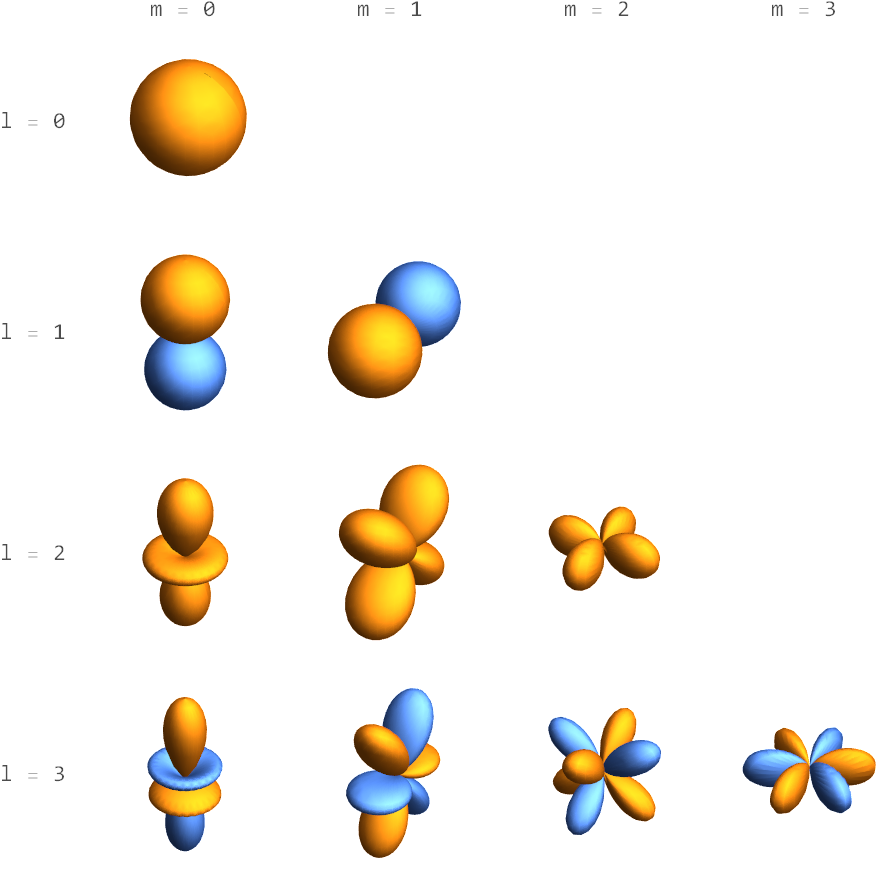
\includegraphics[width=0.5\textwidth]{angle_modes}
            \caption[]{Сферические угловые моды для нескольких $l$}
            \label{fig:angle_modes}
        \end{figure}

        Вскользь затронем вопрос нормировки угловых мод. Для нас данный вопрос не является столь существенным (и далее будет опускаться), однако его рассмотрение имеет целью переход к классической форме записи скалярных мод для демонстрации идентичности результатов, полученных классическими методами и используемой нами методикой.

        Известны т.н. сферические функции $Y_{l,m}(\theta,\varphi)$ вида
        %
        \begin{equation}
            Y_{l,m}(\theta,\varphi) = \frac{1}{\sqrt{2\pi}} \exp(im\varphi) \Theta_{l,m}(\theta) ,
        \end{equation}
        %
        где
        %
        \begin{equation}
            \Theta_{l,m}(\theta) = (-1)^m \sqrt{
                \frac{2l + 1}{2} \frac{(l-m)!}{(l+m)!}
            } P^m_l\qty(\cos\theta) ,
        \end{equation}
        %
        которые образуют полный ортонормированный базис в пространстве функций $f(\theta,\varphi)$, что означает выполнение для них соотношения ортогональности и нормированности на единицу в сферических координатах:
        %
        \begin{equation}
            \braket{Y_{l,m}}{Y_{l',m'}}
                = \int\limits_0^{2\pi} \int\limits_0^\pi {
                    Y_{l,m} Y_{l',m'} \sin\theta
                } \dd{\theta} \dd{\varphi}
                = \delta_{ll'} \delta_{mm'} .
        \end{equation}
        %
        Используем сферические функции в полученном нами результате:
        %
        \begin{equation}
            f_{l,m}(\theta,\varphi)
                = i^m Y_{l,m}(\theta,\varphi) .
        \end{equation}
        %
        Константа $i^m$ здесь не является сколь-нибудь существенной. Действительно, она не влияет на нормировку: $i^m \times (i^m)^* = 1$. Она тем более никак не влияет на ортогональность функций $f_{l,m}$. Поэтому здесь и далее мы будем ее опускать, полагая
        %
        \begin{equation}
            f_{l,m}(\theta,\varphi) \equiv Y_{l,m}(\theta,\varphi) .
        \end{equation}

    %
    %
    %
    %%%%%%%%%%%%%%%%%%%%%%%%%%%%%%%%%%%%%%%%%%%%%%%%%%%%%%%%%%%%%%%%%%%%%%%
    %                           SECTION                                   %
    %%%%%%%%%%%%%%%%%%%%%%%%%%%%%%%%%%%%%%%%%%%%%%%%%%%%%%%%%%%%%%%%%%%%%%%
    %
    %
    %

    \section{Нахождение радиальных частей скалярных сферических мод}

        В данном пункте мы ограничимся скалярными модами $f_{l,m}(r,\theta,\varphi)$.

        Радиальные части сферических мод будем искать из \autoref{eq:wave_equation}. Будем отталкиваться от того, что оператор Лапласа $\Delta$ коммутирует с операторами $\Op{l}^2$ и $\Op{l}_{+} \Op{l}_{-}$, а значит имеет с ними общие собственные функции.

        Поскольку операторы повышения и понижения, $\Op{l}_{+}$ и $\Op{l}_{-}$, не содержат дифференцирования по $r$, искать радиальную часть имеет смысл только для базовой моды. Остальные моды будут иметь точно такую же радиальную часть и получаться из базовой моды путем применения операторов повышения и понижения.

        Решим задачу Штурма-Лиувилля для оператора Лапласа и базовой моды $f_{l}(r,\theta) = f(r) f_{l}(\theta)$:
        %
        \begin{equation}
            \Delta f(r) f_{l}(\theta) = - \lambda f(r) f_{l}(\theta) .
        \end{equation}
        %
        Это дифференциальное уравнение должно выполняться для любого $\theta$. Можно показать, что данное требование выполняется, если $f(r)$ удовлетворяет другому дифференциальному уравнению,
        %
        \begin{equation}
            r^2 f''(r) + 2 r f'(r) + (\lambda r^2 - l(l+1)) f(r) = 0 ,
        \end{equation}
        %
        решением которого являются сферические $J$- и $Y$-функции Бесселя, получаемые из обычных $J$- и $Y$-функций Бесселя по формулам:
        %
        \begin{equation}
            j_n(r) = \frac{\sqrt{\pi/2}}{\sqrt{r}} J_{n+\frac{1}{2}}(r) ; \quad
            y_n(r) = \frac{\sqrt{\pi/2}}{\sqrt{r}} Y_{n+\frac{1}{2}}(r) . \quad
        \end{equation}
        %
        Сферическая $Y$-функция Бесселя, однако, имеет расходимость при $r \to 0$, поэтому не определяет физически реализуемого решения.

        Итак, выбирая единственную константу равной единице, запишем (\autoref{fig:radial_modes})
        %
        \begin{equation}
            f(r) = j_l(\sqrt{\lambda} r) .
        \end{equation}
        %
        Полное решение тогда будет иметь вид:
        %
        \begin{equation}
            f_{l,m}(r,\theta,\varphi)
                = j_l(\sqrt{\lambda} r) Y_{l,m}(\theta,\varphi) .
        \end{equation}
        %
        \begin{figure}[h]
            \centering
            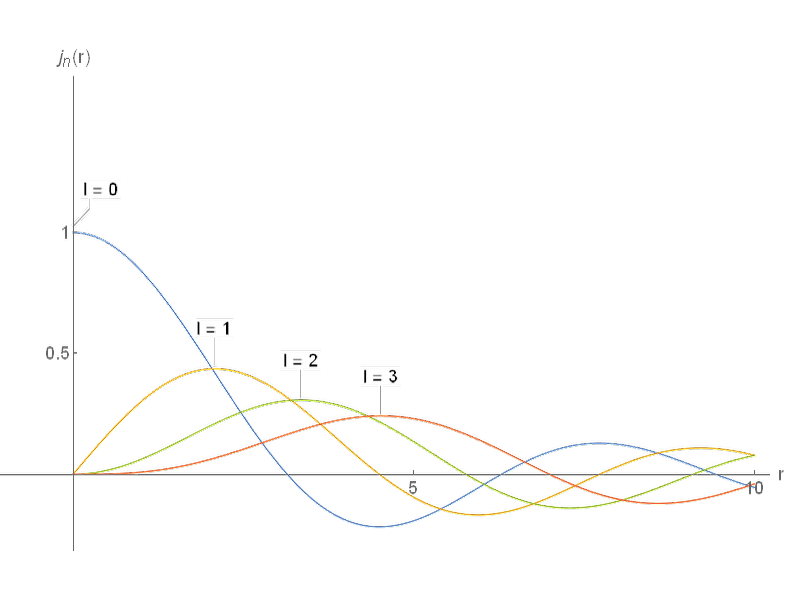
\includegraphics[width=0.5\textwidth]{radial_modes}
            \caption[]{Сферические радиальные моды для нескольких $l$}
            \label{fig:radial_modes}
        \end{figure}

    %
    %
    %
    %%%%%%%%%%%%%%%%%%%%%%%%%%%%%%%%%%%%%%%%%%%%%%%%%%%%%%%%%%%%%%%%%%%%%%%
    %                           SECTION                                   %
    %%%%%%%%%%%%%%%%%%%%%%%%%%%%%%%%%%%%%%%%%%%%%%%%%%%%%%%%%%%%%%%%%%%%%%%
    %
    %
    %

    \section{Векторные сферические моды}

        Применим теперь описанную и проверенную в скалярном случае методику к нахождению сферических мод векторного поля.

        Пусть векторное поле $\vb{a}$ задается своими контравариантными компонентами $a^k$ и удовлетворяет уравнению Лапласа:
        %
        \begin{equation}\label{eq:laplacian_sturm_liouville}
            \Delta \vb{a} = - \lambda \vb{a} .
        \end{equation}

        Для упрощения последующих выкладок и максимального \enquote{развязывания} компонент искомого поля решим следующую задачу. Как известно, базовая мода $\vb{a}_{l,0}$ не зависит от $\varphi$. Найдем разложение $\vb{a}_{l,0}$ на элементарные моды, т.е. моды, имеющие максимальное количество нулевых компонент. Поскольку оператор Лапласа линеен, это вполне допустимо.

        Рассмотрим поле $\vb{b}$ той же конфигурации, что и базовая мода, т.е. $b^k = b^k(r,\theta)$. Будем действовать оператором Лапласа на векторы, получаемые из $\vb{b}$ \enquote{вычеркиванием} отдельных компонент и постановкой на их место нулей, т.е. на $\qty{ b^1, 0, 0 }$, $\qty{ 0, b^2, 0 }$, \dots, $\qty{ 0, b^2, b^3 }$.

        Проделывая эту процедуру в сферических координатах $\qty(r, \theta, \varphi)$, мы обнаружим, что для многих конфигураций поля поставленная задача Штурма-Лиувилля для оператора Лапласа (\autoref{eq:laplacian_sturm_liouville}) в общем нетривиальном случае ($\lambda \neq 0$) неразрешима. Она разрешима лишь для трех конфигураций: $\vb{b}_{\mathrm{I}} = \qty{ b^r, b^\theta, 0 }$, $\vb{b}_{\mathrm{II}} = \qty{ 0, 0, b^\varphi }$ и, собственно, $\vb{b} = \qty{ b^r, b^\theta, b^\varphi } = \vb{b}_{\mathrm{I}} + \vb{b}_{\mathrm{II}}$. Назовем первые две из них $\mathrm{I}$ и $\mathrm{II}$ поляризациями.

        Можно также заметить, что применением операции $\Rot$ одну поляризацию можно \enquote{перевести} в другую, которая тоже будет являться решением волнового уравнения. Это позволяет искать решение только для одной из поляризаций (самой простой), а решение для другой поляризации получать взятием ротора от найденного.

        С точки зрения электродинамики поля $\vb{E}$ и $\vb{H}$ входят в уравнения Максвелла симметрично, вследствие чего оба поля должны удовлетворять одному и тому же волновому уравнению. Поэтому $\vb{H} \sim \Rot{\vb{E}}$ также является решением волнового уравнения. Из данного соотношения можно получить важное следствие: в отдельно взятой элементарно поляризованной моде электромагнитного поля пол\'{я} $\vb{E}$ и $\vb{H}$ имеют \enquote{противоположные} поляризации.

        Применительно к электромагнитному полю конфигурации $\vb{E} = \qty{ E^r, E^\theta, 0 }$ и $\vb{E} = \qty{ 0, 0, E^\varphi }$ называются соответственно\footnotemark{} $TH$ и $TE$.

        \footnotetext{
            Некоторые авторы меняют эти определения местами.
        }

    %
    %
    %
    %%%%%%%%%%%%%%%%%%%%%%%%%%%%%%%%%%%%%%%%%%%%%%%%%%%%%%%%%%%%%%%%%%%%%%%
    %                           SECTION                                   %
    %%%%%%%%%%%%%%%%%%%%%%%%%%%%%%%%%%%%%%%%%%%%%%%%%%%%%%%%%%%%%%%%%%%%%%%
    %
    %
    %

    \section{Нахождение угловых частей векторных сферических мод}

        Найдем угловые части векторных сферических базовых мод. Для краткости обозначим угловую часть базовой $\mathrm{I}$-моды $\vb{a}(\theta)$, а $\mathrm{II}$-моды~--- $\vb{b}(\theta)$.

        Найдем вид $a^k$ и $b^k$, удовлетворяющий \autoref{eq:basemode_op_eq}. Для чего решим полученные из \autoref{eq:basemode_op_eq} дифференциальные уравнения:
        %
        \begin{equation}\begin{aligned}
            l (l + 1) a^1(\theta)
                + \cot(\theta) \partial_\theta a^1(\theta)
                + \partial^2_{\theta\theta} a^1(\theta) &= 0 \\
            (l^2 + l - \csc^2\theta) a^2(\theta)
                + \cot(\theta) \partial_\theta a^2(\theta)
                + \partial^2_{\theta\theta} a^2(\theta) &= 0 \\
            (l^2 + l - 2) b^3(\theta)
                + 3 \cot(\theta) \partial_\theta b^3(\theta)
                + \partial^2_{\theta\theta} b^3(\theta) &= 0
        \end{aligned}\end{equation}

        Решение последнего уравнения в приведенном виде представляет трудности. Оно, однако, допускает сведение к уравнению, по структуре идентичному второму. Представим $b^3(\theta)$ в виде двух множителей: $b^3(\theta) = f(\theta) s(\theta)$. После чего подействуем на $b^k$ оператором повышения и получим:
        %
        \begin{equation}
            \qty(\Op{l}_{+} b^k)^3 = - i \exp(i \varphi) \qty(
                s(\theta) f'(\theta) + f(\theta) \qty(\cot(\theta) s(\theta) + s'(\theta))
            ) .
        \end{equation}
        %
        Сравнивая полученное выражение с
        %
        \begin{equation}
            \qty(\Op{l}_{+} a^k)^1 = - i \exp(i \varphi) \partial_\theta a^1(\theta) ,
        \end{equation}
        %
        выберем $s(\theta)$ так, чтобы
        %
        \begin{equation}
            \cot(\theta) s(\theta) + s'(\theta) = 0 .
        \end{equation}
        %
        Данное соотношение выполняется, если положить $s(\theta) = \csc\theta$.

        Теперь, подставляя $b^k$ в \autoref{eq:basemode_op_eq}, получим дифференциальное уравнение на $f(\theta)$, идентичное уравнению на $a^2$:
        %
        \begin{equation}\label{eq:attached_legendre_pq}
            (l^2 + l - \csc^2\theta) f(\theta) + \cot(\theta) f'(\theta) + f''(\theta) = 0.
        \end{equation}

        Из математической физики известно, что уравнение вида \autoref{eq:attached_legendre_pq} является уравнением на присоединенные полиномы Лежандра первого порядка, $P_l^1(\cos\theta)$ и $Q_l^1(\cos\theta)$. Первое же уравнение уже известно и определяет полиномы Лежандра $P_l(\cos\theta)$ и $Q_l(\cos\theta)$. $Q$-полиномы, однако, не регулярны в нуле, потому не представляют собой физически реализуемого решения.

        Итак, запишем
        %
        \begin{equation}
            \vb{a} = \begin{pmatrix}
                P_l(\cos\theta) \\
                P_l^1(\cos\theta) \\
                0
            \end{pmatrix} , \quad
            \vb{b} = \begin{pmatrix}
                0 \\
                0 \\
                \csc(\theta) P_l^1(\cos\theta)
            \end{pmatrix} .
        \end{equation}

        Получение общего вида производных мод представляет некоторые трудности. Компоненты поля не независимы. После применения оператора повышения (понижения) они \enquote{перемешиваются}, что мешает получению единообразной, пусть даже рекуррентной формулы. Производные моды предлагается искать применением соответствующих операторов. Стоит, однако, отметить, что $m$-я производная мода будет зависеть от $\varphi$ через множитель вида $(-i)^m \exp(i m \varphi)$.

        На \autoref{fig:angle_modes_vect_ii} изображена плотность энергии поля $\vb{b}$. Видно, что она отличается от изображенной на \autoref{fig:angle_modes}. Кроме того, минимальным значением $l$ здесь является $l = 1$ в отличие от скалярного случая, где $l >= 0$.
        %
        \begin{figure}[h]
            \centering
            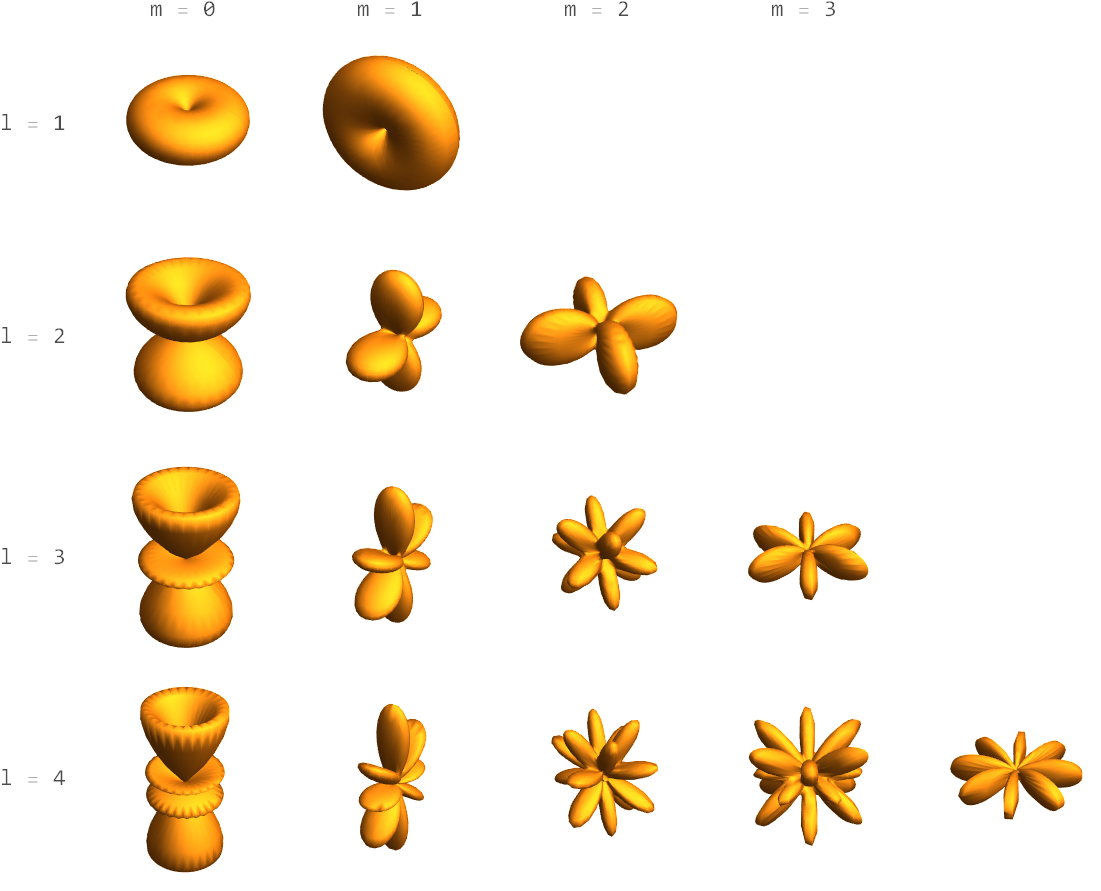
\includegraphics[width=0.5\textwidth]{angle_modes_vect_ii}
            \caption[]{Сферические угловые векторные моды для нескольких $l$}
            \label{fig:angle_modes_vect_ii}
        \end{figure}

    %
    %
    %
    %%%%%%%%%%%%%%%%%%%%%%%%%%%%%%%%%%%%%%%%%%%%%%%%%%%%%%%%%%%%%%%%%%%%%%%
    %                           SECTION                                   %
    %%%%%%%%%%%%%%%%%%%%%%%%%%%%%%%%%%%%%%%%%%%%%%%%%%%%%%%%%%%%%%%%%%%%%%%
    %
    %
    %

    \section{Нахождение радиальных частей векторных сферических мод}

        Как и в скалярном случае, радиальные части сферических мод будем искать из основного уравнения задачи, а именно \autoref{eq:wave_equation}.

        Будем обозначать $\mathrm{I}$-моду как $\vb{a}(r,\theta)$, $\mathrm{II}$-моду~--- как $\vb{b}(r,\theta)$. Напомним, что угловые части $\mathrm{I}$- и $\mathrm{II}$-мод ранее были обозначены как $\vb{a}(\theta)$ и $\vb{b}(\theta)$ соответственно. Итак,
        %
        \begin{equation}\begin{aligned}\label{eq:generic_vector_modes}
            a^i(r,\theta) &= f_i(r) a^i(\theta), \\
            b^i(r,\theta) &= f_i(r) b^i(\theta).
        \end{aligned}\end{equation}
        %
        В выражении выше по $i$ суммирование \textit{не} ведется. Три функции $f_i(r)$, две из которых отвечают двум первым компонентам $\mathrm{I}$-моды, а третья~--- единственной ненулевой компоненте $\mathrm{II}$-моды, будут определены в данном пункте.

        Подстановкой \autoref{eq:generic_vector_modes} в \autoref{eq:wave_equation} получим после необходимых математических преобразований систему уравнений на функции $f_i(r)$:
        %
        \begin{equation}\begin{aligned}
            2 r l (1 + l) f_2(r) + \qty(
                - \qty(2 + l + l^2 - \lambda r^2) f_1(r) +
                2 r f_1'(r) + r^2 f_1''(r)
            ) &= 0, \\
            2 f_1(r) + r \qty(
                - \qty(-2 + l + l^2 - \lambda r^2) f_2(r) +
                4 r f_2'(r) + r^2 f_2''(r)
            ) &= 0, \\
            - \qty(-2 + l + l^2 - \lambda r^2) f_3(r) +
                4 r f_3'(r) + r^2 f_3''(r) &= 0.
        \end{aligned}\end{equation}

        Решением последнего уравнения являются сферические функции Бесселя $l$-го порядка. Первые два уравнения являются сцепленными, и их решение в явном виде представляет трудности. Можно, однако, показать, что совместное решение этих уравнений также имеет результатом сферические функции Бесселя, однако уже смешанных порядков. Можно также получить более простой и естественный вид записи полученных результатов, пользуясь функциями Риккати-Бесселя $S_l(r) = r j_l(r)$. Запишем явный вид $f_i(r)$:
        %
        \begin{equation}\begin{aligned}
            f_1(r) &= \frac{l(l+1)}{r^2} S_l(\sqrt\lambda r), \\
            f_2(r) &= \frac{1}{r^2} S_l'(\sqrt\lambda r) \\
            f_3(r) &= \frac{1}{r^2} S_l(\sqrt\lambda r).
        \end{aligned}\end{equation}
        %
        Штрих в выражении $S_l'(\sqrt\lambda r)$ означает дифференцирование по параметру $\sqrt\lambda r$.

        Таким образом, окончательно имеем:
        %
        \begin{equation}
            \vb{a} = \begin{pmatrix}
                \flatfrac{l(l+1)}{r^2} S_l(\sqrt\lambda r) P_l(\cos\theta) \\
                \flatfrac{1}{r^2} S_l'(\sqrt\lambda r) P_l^1(\cos\theta) \\
                0
            \end{pmatrix} , \quad
            \vb{b} = \begin{pmatrix}
                0 \\
                0 \\
                \flatfrac{1}{r^2} S_l(\sqrt\lambda r) \csc(\theta) P_l^1(\cos\theta)
            \end{pmatrix} .
        \end{equation}

        На \autoref{fig:radial_modes_vect} представлены радиальные части сферических векторных мод разных конфигураций. Заметим, что для $\mathrm{I}$-моды минимальным значением $l$ становится $l = 2$ в виду расходимости $a^2(r,\theta)$ в нуле при меньших значениях параметра.
        %
        \begin{figure}[h]
            \centering
            %
            \subfloat[][]{%
                \label{fig:radial_modes_vect_ib}%
                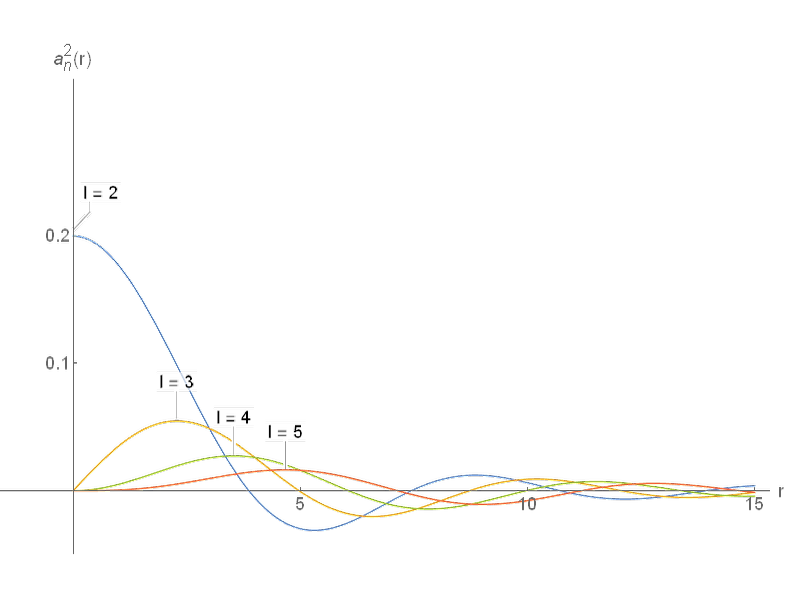
\includegraphics[width=0.45\textwidth]{radial_modes_vect_ib}}%
            \hspace{8pt}%
            %
            \subfloat[][]{%
                \label{fig:radial_modes_vect_ii}%
                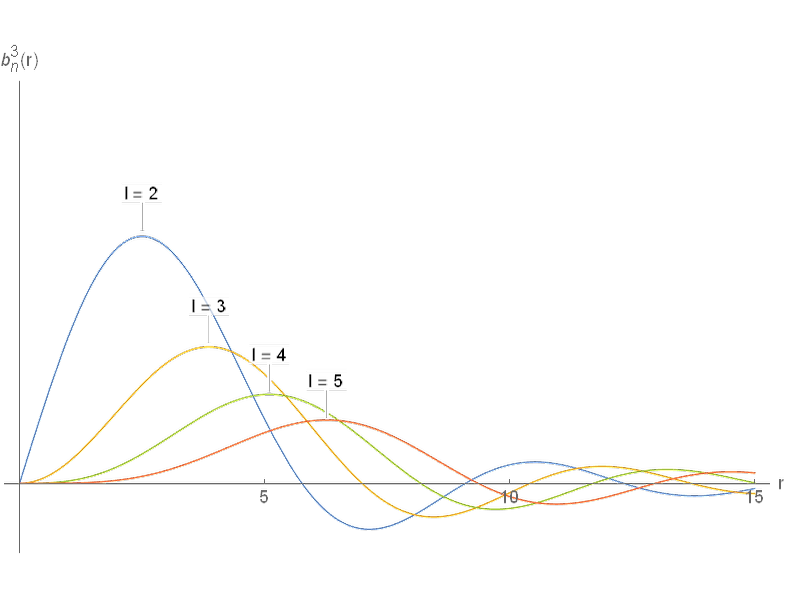
\includegraphics[width=0.45\textwidth]{radial_modes_vect_ii}}%
            \hspace{8pt}%
            %
            \caption[]{Радиальные части векторных сферических мод для нескольких $l$: %
                \subref{fig:radial_modes_vect_ib} вторая компонента $\mathrm{I}$-моды %
                \subref{fig:radial_modes_vect_ii} третья компонента $\mathrm{II}$-моды. %
            } %
            \label{fig:radial_modes_vect}%
        \end{figure}

    %
    %
    %
    %%%%%%%%%%%%%%%%%%%%%%%%%%%%%%%%%%%%%%%%%%%%%%%%%%%%%%%%%%%%%%%%%%%%%%%
    %                           SECTION                                   %
    %%%%%%%%%%%%%%%%%%%%%%%%%%%%%%%%%%%%%%%%%%%%%%%%%%%%%%%%%%%%%%%%%%%%%%%
    %
    %
    %

    \section{Условия на поверхности резонатора}

        Ранее мы не поднимали вопрос о граничных условиях, пользуясь лишь знанием о сферической симметрии задачи. Теперь встает вопрос их учета.

        Для начала снова поговорим о волновом уравнении (\autoref{eq:wave_equation}). Оно является задачей Штурма-Лиувилля для оператора Лапласа. Ранее мы ввели обозначение для собственного значения оператора Лапласа, взятого с обратным знаком: $\lambda = \varepsilon \flatfrac{\omega^2}{c^2}$. Оно является функцией частоты и определяет масштаб переменной $r$ в радиальных частях сферических мод, поэтому определяется граничными условиями задачи. Это, в свою очередь, означает, что спектр возможных энергий является дискретным, т.е. возможны лишь частоты $\omega_n$, $n = 1, 2, \dots$. Выясним, чем они определяются.

        Граничные условия в идеальном случае должны обеспечивать отсутствие потока энергии через поверхность резонатора и отсутствие поверхностных токов. Для отсутствия поверхностных токов необходимо, чтобы тангенциальные составляющие поля $\vb{E}$ обращались в нуль. Покажем, что этого достаточно также и для обращения в нуль потока энергии.

        Поток энергии $\Phi$ и плотность потока энергии $\vb{S}$ (вектор Умова-Пойнтигна) даются выражениями:
        %
        \begin{equation}\begin{gathered}
            \Phi = \oint_\Omega \vb{S} \dd{\vb{\Omega}}
                 = \oint_\Omega S_r \dd{\Omega} , \\
            \vb{S} = \vb{E} \times \vb{H} .
        \end{gathered}\end{equation}
        %
        Вклад в поток энергии через границу резонатора вносит только радиальная составляющая плотности потока $S_r = \vb{S} \cdot \vb{e}_r$. Вычислим ее в общем случае, представив поля $\vb{E}$ и $\vb{H}$ в виде разложения по базису $\qty{ \vb{e}_r, \vb{e}_\theta, \vb{e}_\varphi }$. В силу ортогональности и нормированности базиса $\vb{e}_i$ все произведения вида $\vb{e}_j \times \vb{e}_k$ либо равны нулю ($j = k$), либо дают вектор $\pm \vb{e}_{i \neq j,k}$. Вектор $\vb{e}_r$, таким образом, получается из произведения двух тангенциальных базисных векторов: $\vb{e}_\theta \times \vb{e}_\varphi = \vb{e}_r$.

        Итак, в $S_r$ дают вклад только перекрестные произведения тангенциальных компонент полей $\vb{E}$ и $\vb{H}$, т.е.
        %
        \begin{equation}
            S_r = E_\theta H_\varphi - H_\theta E_\varphi .
        \end{equation}
        %
        Для каждой из поляризаций поля $\vb{E}$ останется только одно слагаемое~--- первое для $\mathrm{I}$ поляризации и второе для $\mathrm{II}$ поляризации. Однако равенство нулю тангенциальных компонент поля $\vb{H}$ не совместно с равенство нулю тангенциальных компонент поля $\vb{E}$, что является необходимым условием отсутствия поверхностных токов. Поэтому граничные условия выражаются в требовании исчезновения у поля $\vb{E}$ тангенциальных составляющих на поверхности резонатора.

        Ранее было показано, что радиальные функции являются комбинациями из функций Бесселя от аргумента $\sqrt\lambda r$. Отсюда мы можем заключить, что спектр собственных частот резонатора является последовательностью $\omega_n = \omega_n(\lambda_n)$, где $\lambda_n$ определяется из условия равенства нулю радиальной составляющей касательной части поля $\vb{E}$ на поверхности резонатора, т.е. при $r = r_\text{шара}$.

    %
    %
    %
    %%%%%%%%%%%%%%%%%%%%%%%%%%%%%%%%%%%%%%%%%%%%%%%%%%%%%%%%%%%%%%%%%%%%%%%
    %                        BIBLIOGRAPHY                                 %
    %%%%%%%%%%%%%%%%%%%%%%%%%%%%%%%%%%%%%%%%%%%%%%%%%%%%%%%%%%%%%%%%%%%%%%%
    %
    %
    %

    \nocite{*}
    \bibliographystyle{../../lib/doc/bib/utf8gost705s}
    \bibliography{../../lib/doc/bib/physics,math}

\end{document}
